\documentclass[11pt,a4paper]{article}

\usepackage[polish]{babel}
\usepackage{polski}
\usepackage[utf8]{inputenc}
\usepackage[T1]{fontenc}
\usepackage{graphicx}
\usepackage{color}
\usepackage{placeins}
\usepackage[math]{anttor}
\usepackage{natbib}
\frenchspacing

\newcommand{\todo}[1]{\colorbox{yellow}{#1}}

\begin{document}

\title{Automatyczna klasyfikacja i ekstrakcja tematu krótkich notatek w języku polskim}
\author{Paweł Obrok\\pod kierunkiem dr. Michała Korzyckiego}

\maketitle
\pagebreak

\tableofcontents
\pagebreak

\section{Wstęp}
\section{Podstawy teoretyczne}
\section{Procedura badawcza}
\section{Opis danych}
\subsection{Przykładowy problem}
\label{sec:example}
\section{Wyniki i analiza}

Niniejszy rozdział zawiera porównanie różnych aspektów działania algorytmów LDA
i LSI. Na jego końcu znajdują się wnioski jakie można wyciągnąć z zebranych
danych.

\subsection{Tematy}

Tabele \ref{fig:lsi_topics} i \ref{fig:lda_topics} zawierają niektóre tematy
wygenerowane przez algorytmy LSI i LDA skonfigurowane na 100 tematów (po
dziesięć najbardziej znaczących słów w każdym temacie). Pojedynczy wiersz
tabeli zawiera jeden temat - liczby przy tokenach oznaczają wagi poszczególnych
słów w danym temacie.

Tematy uzyskane przy pomocy LDA wydają się bardziej odpowiadać postrzeganiu
tekstu przez człowieka niż te wygenerowane przez LSI.  Przykładowo temat numer 4 w tabeli
\ref{fig:lsi_topics} można interpretować jako ,,nie pogoda i finanse`` ---
możliwość złożenia dwóch tematów postrzeganych przez człowieka w jeden, ale z
przeciwnymi znakami powoduje powstawanie tego typu kombinacji. Tematy wygenerowane
przez LDA bywają złożeniami dwóch różnych konceptów, jednak zawsze mają ten sam znak,
jak na przykład temat numer 5 w tabeli \ref{fig:lda_topics}, który wydaje się łączyć
koncepty ,,muzeum`` i ,,przestępstwo``.

\begin{table}[h]
\label{fig:lsi_topics}
\caption{Tematy wyekstrahowane przez algorytm LSI}
\begin{tabular}{|c|p{\linewidth}|}
\hline
Lp. & Temat \\\hline
1 & 0.269*" + 0.181*- + 0.171*być + 0.161*procent + 0.144*polski + 0.138*rok + 0.119*) + 0.118*złoty + 0.111*( + 0.102*a \\\hline
2 & -0.304*procent + -0.265*wzróść + -0.254*punkt + -0.211*WIG + -0.192*wynieść + -0.191*spaść + -0.180*złoty + -0.165*spółka + -0.158*akcja + 0.158*" \\\hline
3 & 0.482*RATIO + 0.265*mecz + 0.234*: + 0.187*pokonać + 0.182*mistrzostwo + 0.149*) + 0.149*turniej + -0.142*" + 0.119*piłkarski + 0.117*wygrać \\\hline
4 & -0.301*stopień + -0.250*temperatura + -0.240*maksymalny + -0.228*wiatr + -0.222*umiarkowany + -0.216*deszcz + -0.212*słaby + -0.208*opad + -0.181*południe + 0.164*złoty \\\hline
5 & -0.390*złoty + -0.305*grosz + -0.262*dolar + -0.246*euro + 0.210*punkt + -0.195*osiągać + -0.170*milion + 0.159*WIG + -0.147*umocnić + 0.142*procent \\\hline
6 & -0.355*spółka + -0.301*Akcyjna + 0.259*grosz + -0.223*milion + 0.215*zamknięcie + 0.185*euro + 0.180*osiągać + 0.170*punkt + 0.153*dolar + -0.148*bank \\\hline
7 & -0.435*procent + 0.300*spółka + -0.232*rok + 0.212*akcja + -0.191*proca + 0.190*Akcyjna + 0.148*giełda + -0.133*milion + 0.127*zmienić + 0.124*kurs \\\hline
8 & -0.227*RATIO + 0.192*sąd + -0.147*: + 0.147*( + -0.135*unia + -0.129*mecz + 0.127*policja + -0.125*spółka + 0.122*tysiąc + -0.122*AWS \\\hline
9 & 0.313*( + 0.274*) + -0.258*RATIO + -0.165*mecz + -0.158*sąd + -0.144*: + 0.133*wyścig + 0.126*mistrzostwo + 0.120*spółka + 0.120*świat \\\hline
10 & -0.230*sąd + 0.220*europejski + -0.187*AWS + 0.154*unia + -0.148*procent + 0.143*UE + -0.119*wyborczy + -0.118*okręgowy + 0.114*polski + 0.111*milion \\\hline
\end{tabular}
\end{table}

\begin{table}[h]
\label{fig:lda_topics}
\caption{Tematy wyekstrahowane przez algorytm LDA}
\begin{tabular}{|c|p{\linewidth}|}
\hline
Lp. & Temat \\\hline
1 & 0.027*open + 0.026*powodzianin + 0.021*podlaski + 0.018*Słowenia + 0.017*cukrownia + 0.017*najstarszy + 0.013*przedstawiony + 0.012*urodziny + 0.012*rata + 0.012*zrezygnować\\\hline
2 & 0.021*europejski + 0.021*unia + 0.018*UE + 0.012*polski + 0.011*kraj + 0.010*" + 0.009*Litwa + 0.009*unijny + 0.008*państwo + 0.008*NATO\\\hline
3 & 0.032*palestyński + 0.031*Izrael + 0.030*izraelski + 0.023*Palestyńczyk + 0.015*Arafat + 0.013*szaron + 0.013*świętokrzyski + 0.012*zawieszenie + 0.012*autonomia + 0.011*arabski\\\hline
4 & 0.024*sąd + 0.015*aresztować + 0.015*podejrzany + 0.014*rejonowy + 0.013*okręgowy + 0.013*śledczy + 0.013*akt + 0.012*Gdynia + 0.012*oskarżenie + 0.012*Radom\\\hline
5 & 0.016*wierzyciel + 0.013*muzeum + 0.013*wystawa + 0.011*zbiór + 0.011*śląski + 0.011*Brazylijczyk + 0.010*łączny + 0.010*zajmujący + 0.009*przestępczy + 0.009*łódzki\\\hline
6 & 0.032*festiwal + 0.022*woj + 0.017*Białystok + 0.017*letni + 0.014*wielkopolski + 0.014*wrzesień + 0.014*kupno + 0.012*ogólnopolski + 0.012*usuwanie + 0.012*impreza\\\hline
7 & 0.019*siatkarz + 0.011*obniżka + 0.009*noc + 0.007*postać + 0.006*Gorzów + 0.006*artystyczny + 0.006*bóg + 0.006*bandyta + 0.005*nieznany + 0.005*ZSRR\\\hline
8 & 0.012*" + 0.011*general + 0.010*motors + 0.008*Jedwabne + 0.008*kardynał + 0.007*film + 0.007*weekend + 0.007*Józef + 0.007*rocznica + 0.006*odbyć\\\hline
9 & 0.017*świat + 0.016*klasa + 0.016*TP + 0.015*metr + 0.015*( + 0.015*) + 0.014*mistrzostwo + 0.014*zająć + 0.013*AZS + 0.013*bieg\\\hline
10 & 0.044*obligacja + 0.021*Artur + 0.018*włosek + 0.017*pomnik + 0.016*politechnika + 0.016*białostocki + 0.016*społeczność + 0.013*wyeliminować + 0.012*skorzystać + 0.011*wyemitować\\\hline
\end{tabular}
\end{table}

\FloatBarrier

\subsection{Czas działania}

\todo{Czy to ma sens?}

\subsection{Metryki z nadzorem}

W tym rozdziale omówiono wyniki otrzymane za pomocą algorytmów LDA i LSI dla
przykładowego problemu opisanego w \ref{sec:example}. Należy zauważyć, że tego
rodzaju ewaluacja wymaga ręcznego przygotowania danych testowych przez
człowieka, co może być nieprakyczne dla dużych zbiorów danych.  Jej zaletą jest
fakt, że mierzy ona faktyczne osiągi danego rozwiązania w rzeczywistych
problemach.

\subsubsection{Ranking dokumentów}

Wykresy \ref{ranks_stemming_comparison} i \ref{ranks_no_stemming_comparison}
przedstawiają sumę kwadratów ranków dokumentów z wzorca przygotowanego ręcznie
dla danego zapytania w wynikach działania odpowiednio algorytmów LDA i LSI dla
różnej liczby tematów.

Algorytm LDA osiąga ogólnie gorsze wyniki niż LSI - poza przedziałem $50 - 100$
tematów. Gorszy jest też (aczkolwiek niewiele) najlepszy wynik jaki udałoby się
osiągnąć odpowiednio dobierając liczbę tematów. Na wykresie daje się także
zauważyć stochastyczna natura LDA - podczas gdy dla LSI wyniki niemal
monotonicznie poprawiają się wraz ze wzrostem liczby tematów dla LDA zdarza się
znaczne pogorszenie wyników przy zwiększeniu tej liczby.

Polepszenie wyników dzięki zastosowaniu stemmingu jest widoczne na pierwszy
rzut oka --- polski jako język silnie fleksyjny jest znakomitym kandydatem do
zastosowania tego typu techniki. W \cite{manning-schuetze} zasugerowano, że ze
stemmingu można zrezygnować dyponując odpowiednio dużym zbiorem danych jednak
wyniki te uzyskano dla języka angielskiego, którego fleksja jest znacznie mniej
rozbudowana. W tym wypadku zebranie tak dużej ilości danych może być mniej
praktyczne niż skonstruowanie słownika fleksyjnego takiego jak na przykład ten
opisany w \cite{pisarek-slownik}.

Co ciekawe algorytm LDA radzi sobie znacznie lepiej od LSI bez wykorzystania
stemmingu.  Może to być spowodowane trudnością w przypadku LSI połączenia ze
sobą słów, które różnią się formą fleksyjną i są w tym wypadku traktownae
całkowicie osobno.

\begin{figure}[h]
\caption{Suma kwadratów ranków dokumentów ze wzorca dla testowego zapytania (z wykorzystaniem stemmingu)}
\label{ranks_stemming_comparison}
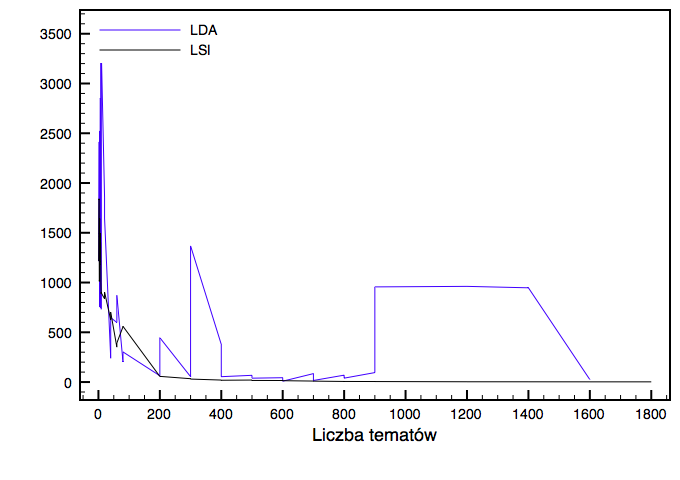
\includegraphics[width=\linewidth]{gfx/ranks_stemming.png}
\end{figure}

\begin{figure}[h]
\caption{Suma kwadratów ranków dokumentów ze wzorca dla testowego zapytania (bez wykorzystania stemmingu)}
\label{ranks_no_stemming_comparison}
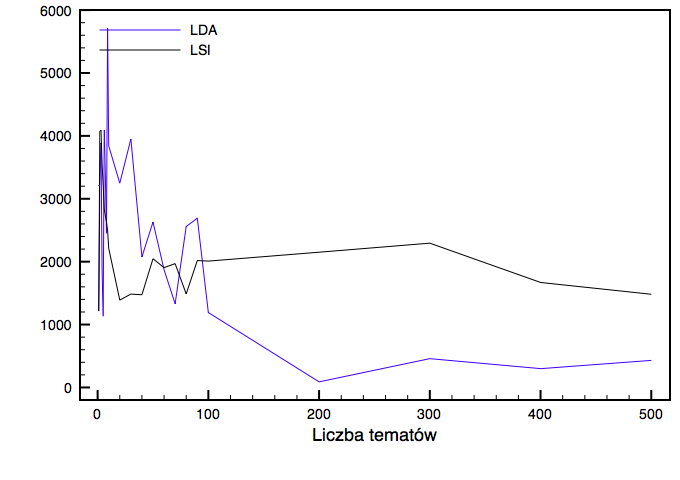
\includegraphics[width=\linewidth]{gfx/ranks_no_stemming.png}
\end{figure}

\FloatBarrier

\subsubsection{Krzywe ROC}

Krzywa ROC \cite{roc-article1} (Receiver Operation Characteristic) to wykres
przedstawiający dla danego klasyfikatora zależność między stosunkiem liczby
znalezionych dokumentów relewantnych do liczby wszystkich zwróconych dokumentów
(TPR --- True Positive Rate), a stosunkiem liczby odrzuconych dokumentów
relewantnych do liczby wszystkich odrzuconych dokumentów (FPR - False Positive
Rate) w miarę zmiany progu detekcji. W tym wypadku ten zmienny próg to po
prostu liczba $n$ - pierwszych $n$ dokumentów jest traktowane jako odnalezione,
a pozostałe jako odrzucone.

Lepsze klasyfikatory charakteryzują się krzywymi ROC położonymi dalej od linii
$x = y$.  Klasyfikatory blisko, lub na tej linii nie wykonują żadnej użytecznej
pracy. Analiza odległości krzywej ROC od linii $x = y$ w różnych miejscach
wykresu może dać wskazówkę co do najlepszego dobrania progu detekcji dla danego
problemu.

Wykresy \ref{roc_lsi} i \ref{roc_lda} przedstawiają krzywe ROC dla algorytmów
LDA i LSI dla różnych liczb tematów. Dla dużych liczb tematów algorytm LDA
spisuje się gorzej, jednak można zauważyć, że klasyfikator uzyskany dla 30
tematów jest podobnej jakości lub lepszy jak ten uzyskany przy użyciu LSI dla
100 tematów.

\begin{figure}[h]
\caption{Krzywe ROC dla algorytmu LSI dla wybranych liczb tematów}
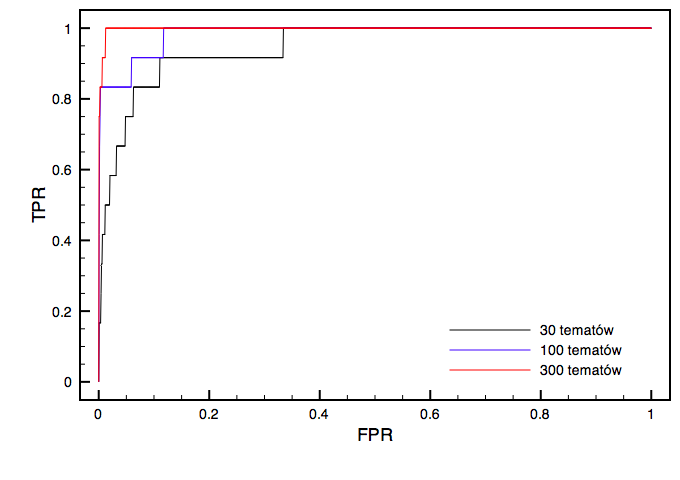
\includegraphics[width=\linewidth]{gfx/lsi_roc.png}
\label{roc_lsi}
\end{figure}

\begin{figure}[h]
\caption{Krzywe ROC dla algorytmu LDA dla wybranych liczb tematów}
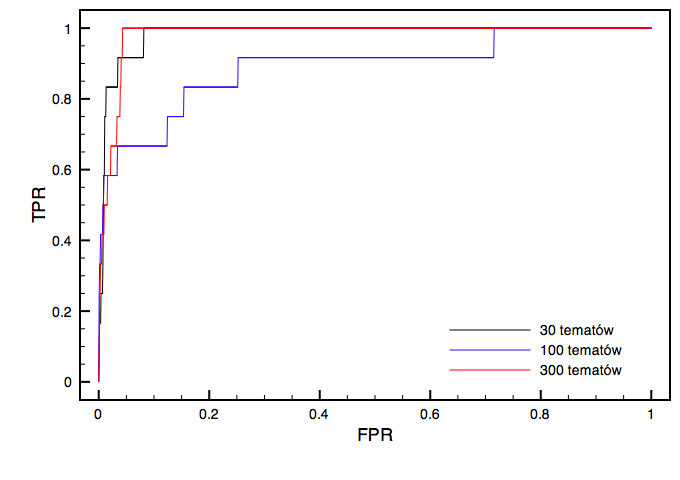
\includegraphics[width=\linewidth]{gfx/lda_roc.png}
\label{roc_lda}
\end{figure}

Na wykresach \ref{roc_lsi_untagged} i \ref{roc_lda_untagged} przedstawione
zostały krzywe ROC dla algorytmów LSI i LDA bez wykorzystania stemmingu.
Ponownie daje się zauważyć lepsze działanie algorytmu LDA w tym wypadku -
klasyfikator uzyskany dla 300 tematów jest znacznie lepszy od tego uzyskanego
przy pomocy LSI.

\begin{figure}[h]
\caption{Krzywe ROC dla algorytmu LSI dla wybranych liczb tematów bez wykorzystania stemmingu}
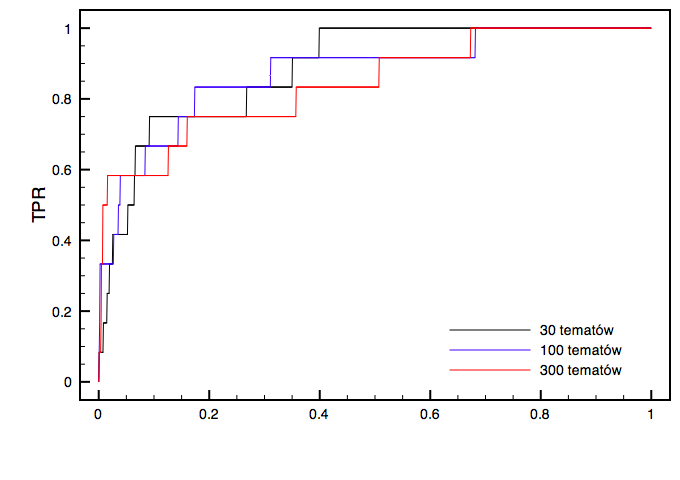
\includegraphics[width=\linewidth]{gfx/lsi_roc_untagged.png}
\label{roc_lsi_untagged}
\end{figure}

\begin{figure}[h]
\caption{Krzywe ROC dla algorytmu LDA dla wybranych liczb tematów bez wykorzystania stemmingu}
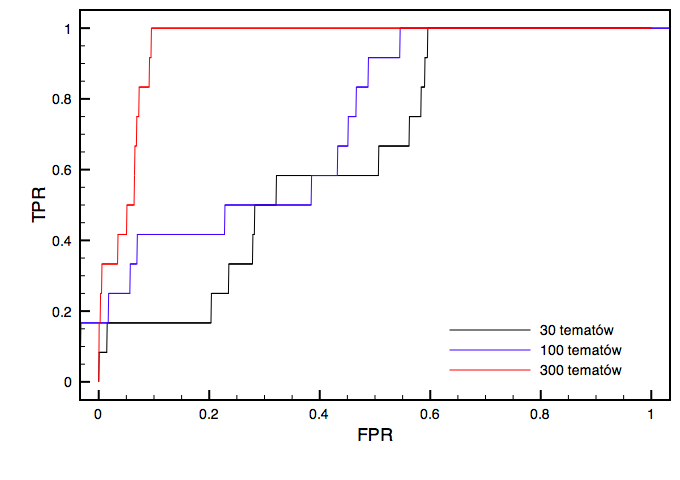
\includegraphics[width=\linewidth]{gfx/lda_roc_untagged.png}
\label{roc_lda_untagged}
\end{figure}

\FloatBarrier

\subsubsection{Przywołanie i precyzja}

Przywołanie (stosunek liczby zwróconych relewantnych dokumentów do liczby
wszystkich relewantncyh dokumentów) i prezycja (stosunek liczby zwróconych
relewantncyh dokumentów do liczby wszystkich zwróconych dokumentów) to częste
metryki w zadaniach typu information retrieval. Wybranie jakiegoś poziomu
przywołania reprezentuje pewien kompromis między kompletnością zwróconych
danych, a częstością występowania w nich danych relewantnych, a więc ilością
czasu, które musi poświęcić operator systemu na ich dalsze przetworzenie.

Wykresy \ref{fig:lsi_precision} i \ref{fig:lda_precision} prezentują precyzę
osiąganą przez algorytmy LDA i LSI na różnych poziomach przywołania dla
przykładowego problemu.

Można zauważyć, że LDA daje znacznie gorszą precyzję niż LSI. Nawet najlepiej
dobrana liczba tematów (w tym wypadku 300) pozwala osiągać precyzję
porównywalną jedynie z LSI dla 30 tematów.

\begin{figure}[h]
\caption{Precyzja na różnych poziomach przywołania dla algorytmu LSI}
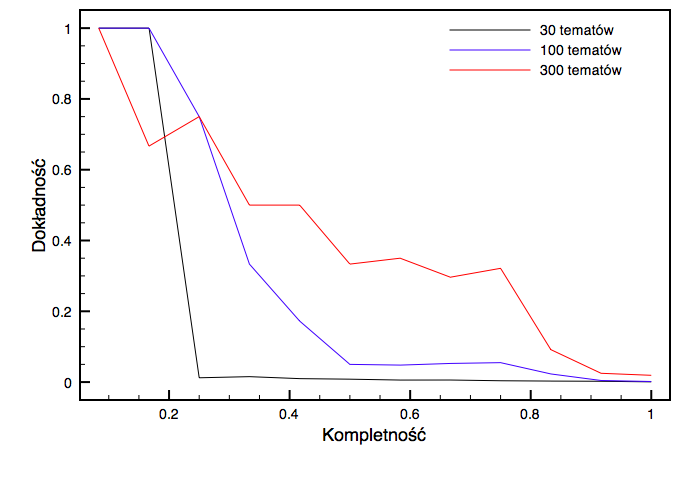
\includegraphics[width=\linewidth]{gfx/lsi_precision.png}
\label{fig:lsi_precision}
\end{figure}

\begin{figure}[h]
\caption{Precyzja na różnych poziomach przywołania dla algorytmu LDA}
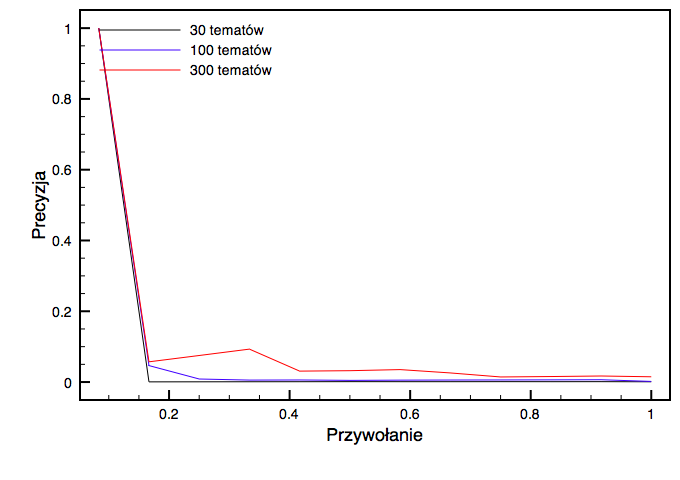
\includegraphics[width=\linewidth]{gfx/lda_precision.png}
\label{fig:lda_precision}
\end{figure}

\FloatBarrier

\subsection{Metryki bez nadzoru (perplexity)}

Współczynnik perplexity, którego wartości w zależności od liczby tematów są
przedstawione na wykresie \ref{fig:perplexity}, daje pewne pojęcie o tym jak
dobrze model jest w stanie przewidzieć nowe dane. Wysokie wartości
współczynnika mogą wskazywać, że model jest przeuczony i będze słabo uogólniał
swoje działania na nieznane dane. Jest on dobrym wskaźnikiem jak dobrze dany
model będzie sobie radził z klastrowaniem danego zbioru danych.

Wykres demonstruje, że optymalne wartości współczynnika perplexity zostają
osiągnięte w okolicach 50 tematów. W tym wypadku może to sugerować, że mniej
więcej na tyle właśnie grup tematycznych należałoby podzielić ten zbiór danych.

Algorytm LDA zachowuje niski współczynnik perplexity tylko stosunkowo blisko
optymalnej liczby tematów. Takie zachowanie może wymagać dokładnego strojenia
algorytmu do każdego zastosowania, co bywa uciążliwe i czasochłonne.

\begin{figure}[h]
\caption{Współczynnik perplexity dla LDA i LSI w zależności od liczby tematów}
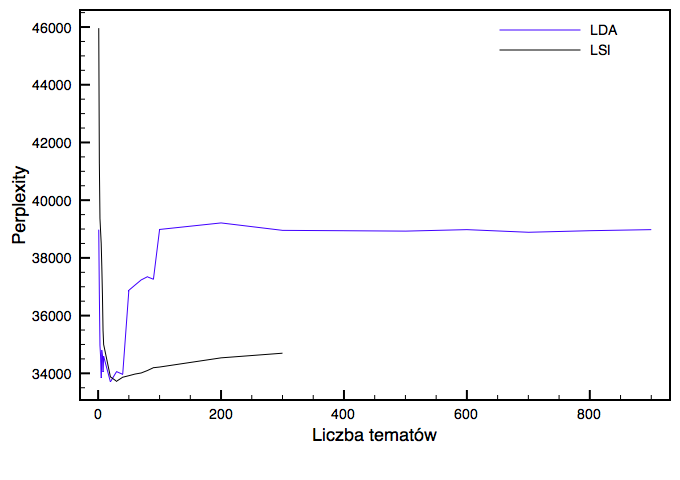
\includegraphics[width=\linewidth]{gfx/perplexity.png}
\label{fig:perplexity}
\end{figure}

\FloatBarrier

\subsection{Wnioski}

Algorytm LDA daje gorszej jakości (a przynajmniej mniej stabilne) wyniki dla
typowych problemów klasyfikacji i wyszukiwania informacji spotykanych w
codziennej praktyce. Wydaje się za to być w stanie działać w sytuacji, gdy
wiele różnych tokenów oznacza to samo (przypadek bez wykorzystania stemmingu),
w odróżnieniu od LSI, którego wyniki są wtedy całkowicie nieprzydatne. To
bardzo porządana cecha w przypadku braku odpowiedniego słownika fleksyjnego dla
danego języka.

Przewagą LDA wydaje się być jakość generowanych tematów --- przez wymuszenie
dodatnich wag otrzymujemy na najbardziej znaczących pozycjach (z najwyższymi
wagami) słowa opisujące dany dokument/temat, podczas gdy w przypadku LSI mogą
to być słowa najodleglejsze. Takie zachowanie może okazać się korzystne w
zastosowaniach typu tagowanie dokumentów lub automatyczne generowanie
podsumowań czy słów kluczowych.

\section{Podsumowanie}

\bibliographystyle{abbrv}
\bibliography{thesis}

\enddocument
